\section{Testbench Architecture}

\begin{figure}[htb]
 \centering
 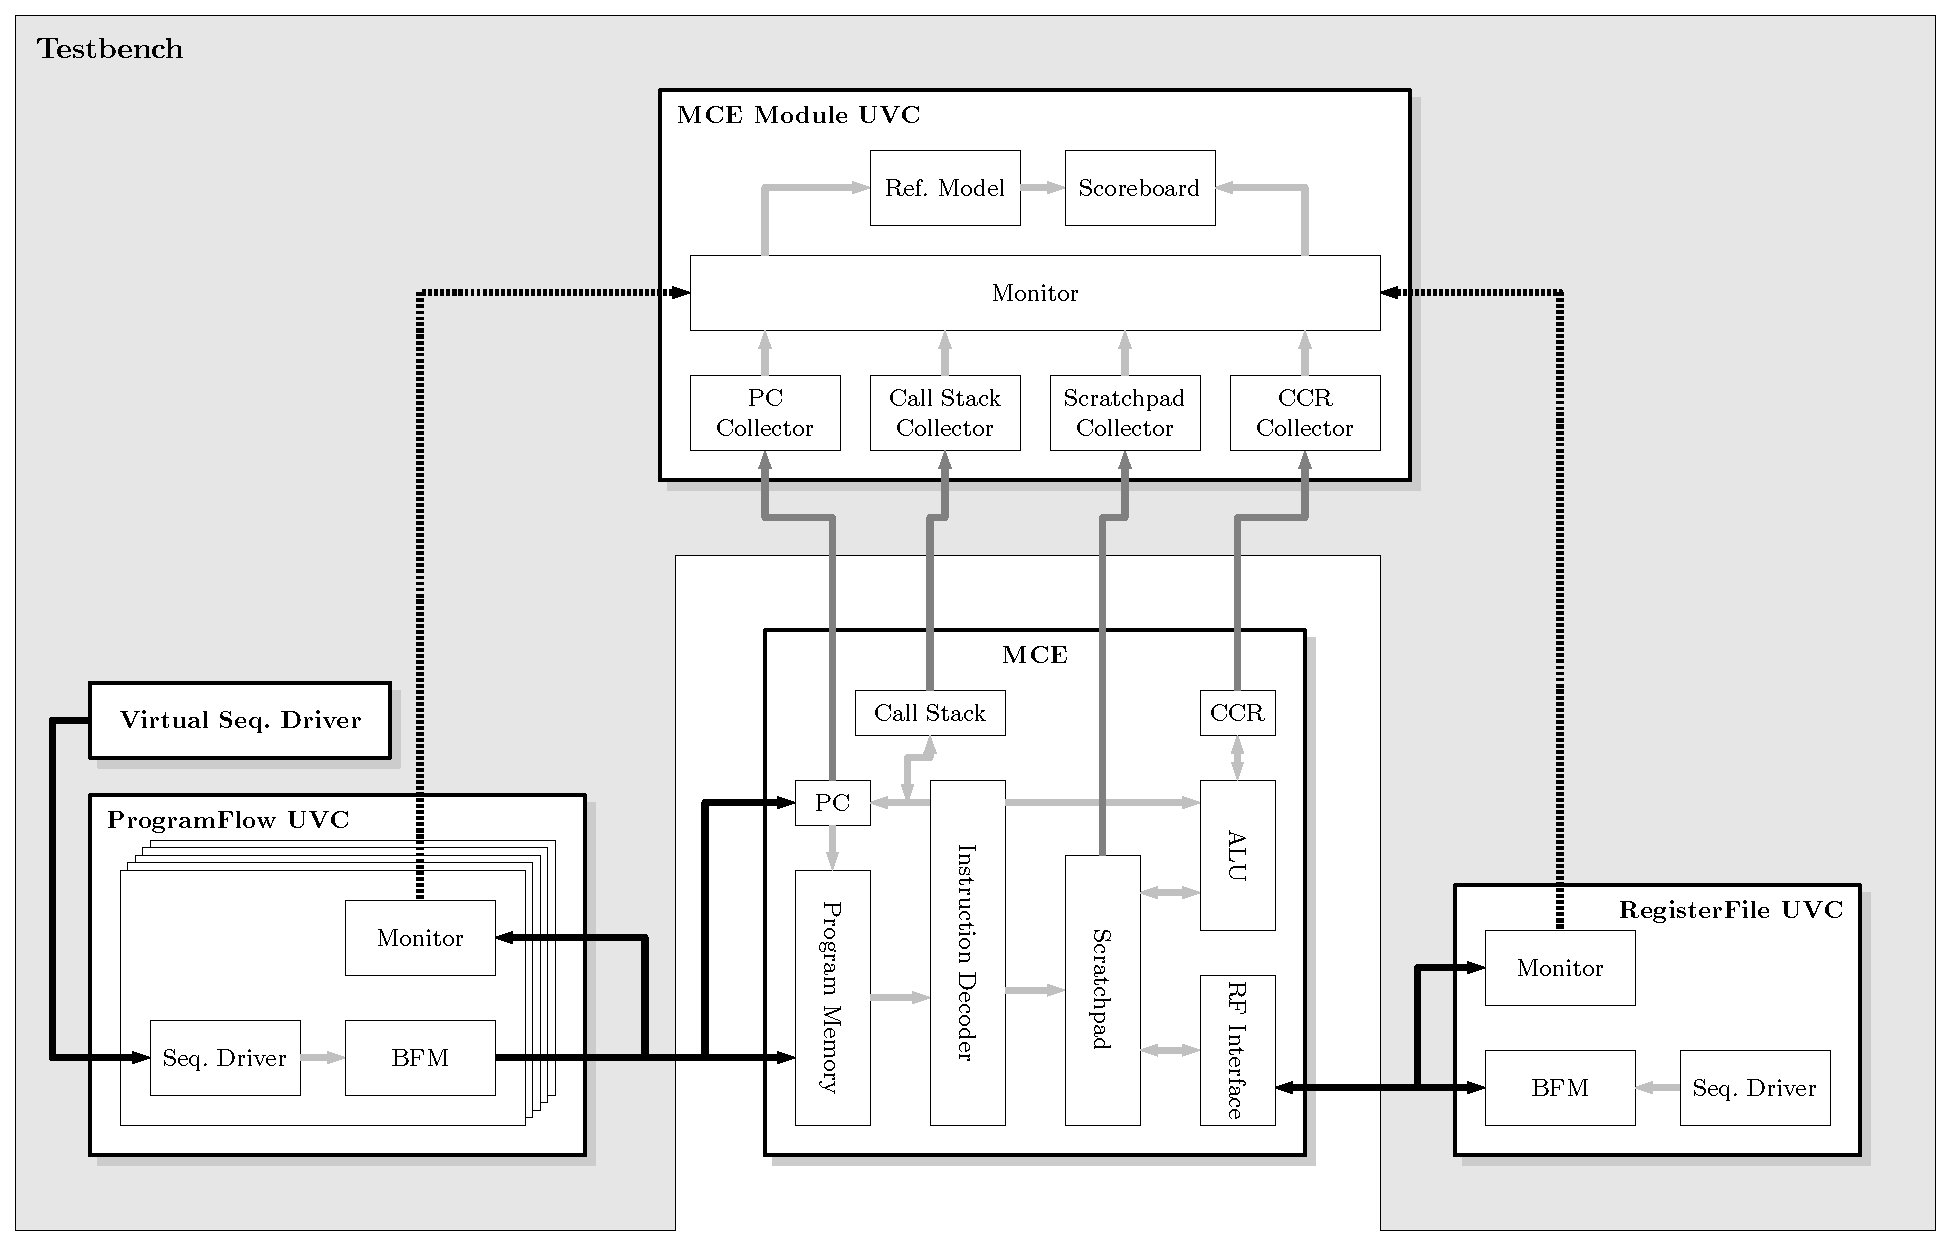
\includegraphics[width=1.0\textwidth,angle=0]{images/mce_tb}
 \caption{MCE Testbench}
\label{fig:mce_tb}
\end{figure}

\subsection{ProgramFlow Inteface UVC}

\subsubsection{Program Memory Agent}

\subsubsection{External Condition Code Bits Agent}

\subsubsection{Call Stack Overflow Agent}

\subsubsection{Start Agent}

\subsubsection{Done Agent}

\subsection{RegisterFile Interface UVC}

\subsection{MCE Module UVC}

\begin{figure}[htb]
 \centering
 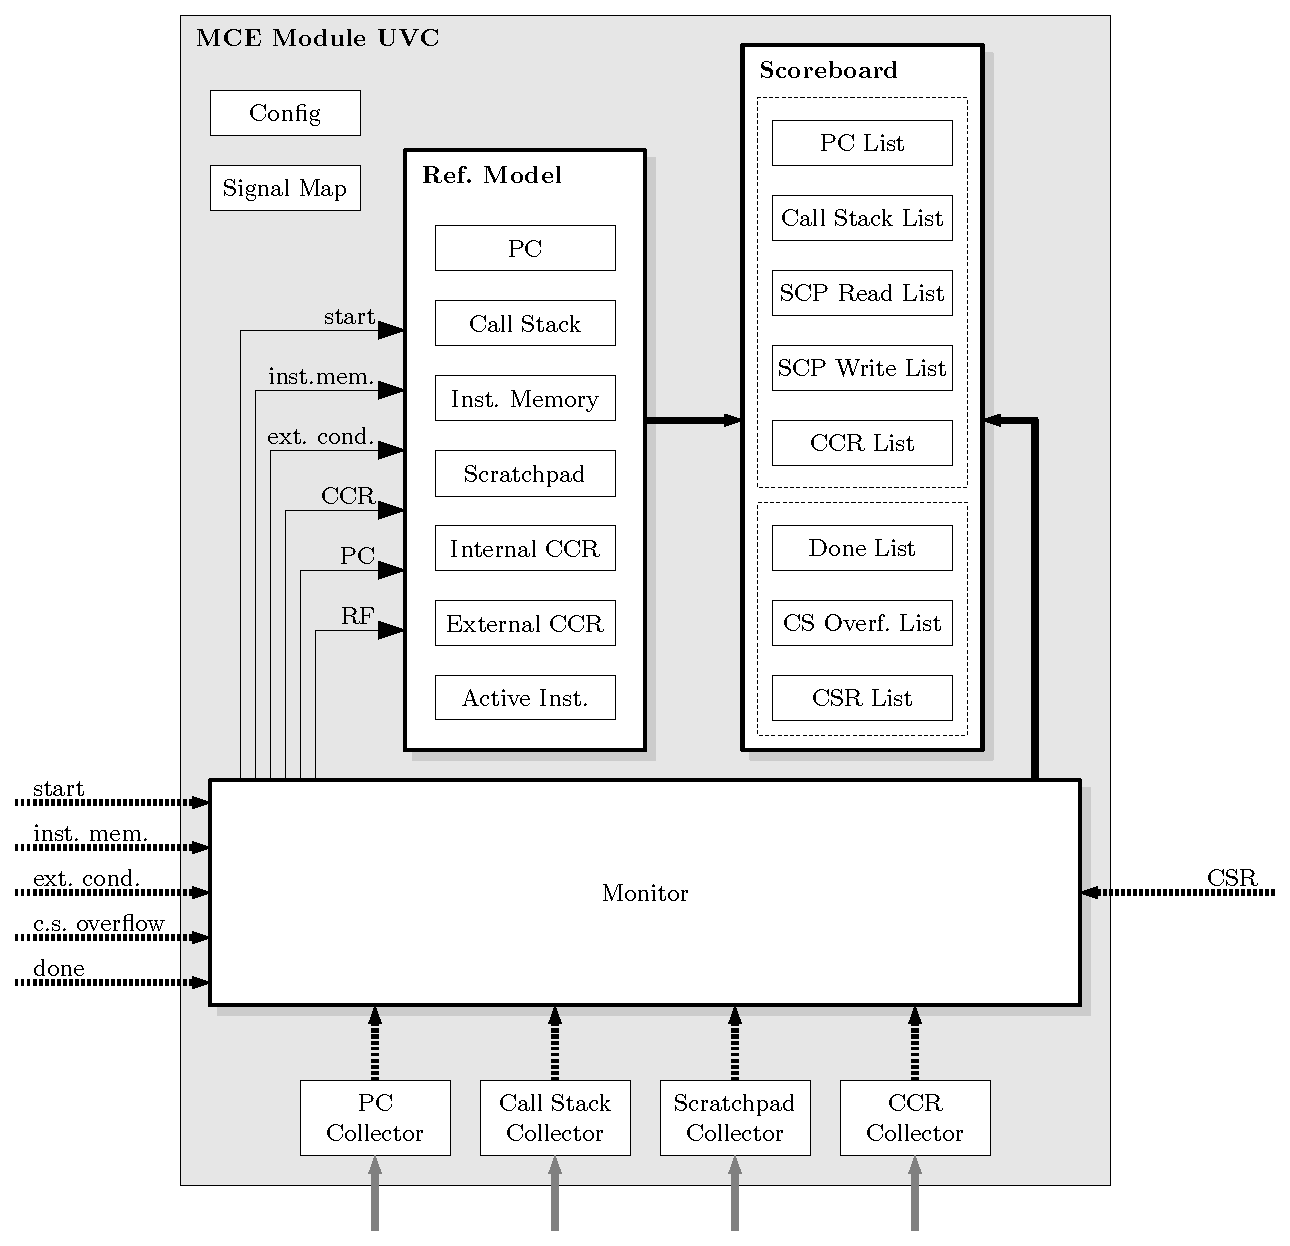
\includegraphics[width=1.0\textwidth,angle=0]{images/mce_module_uvc}
 %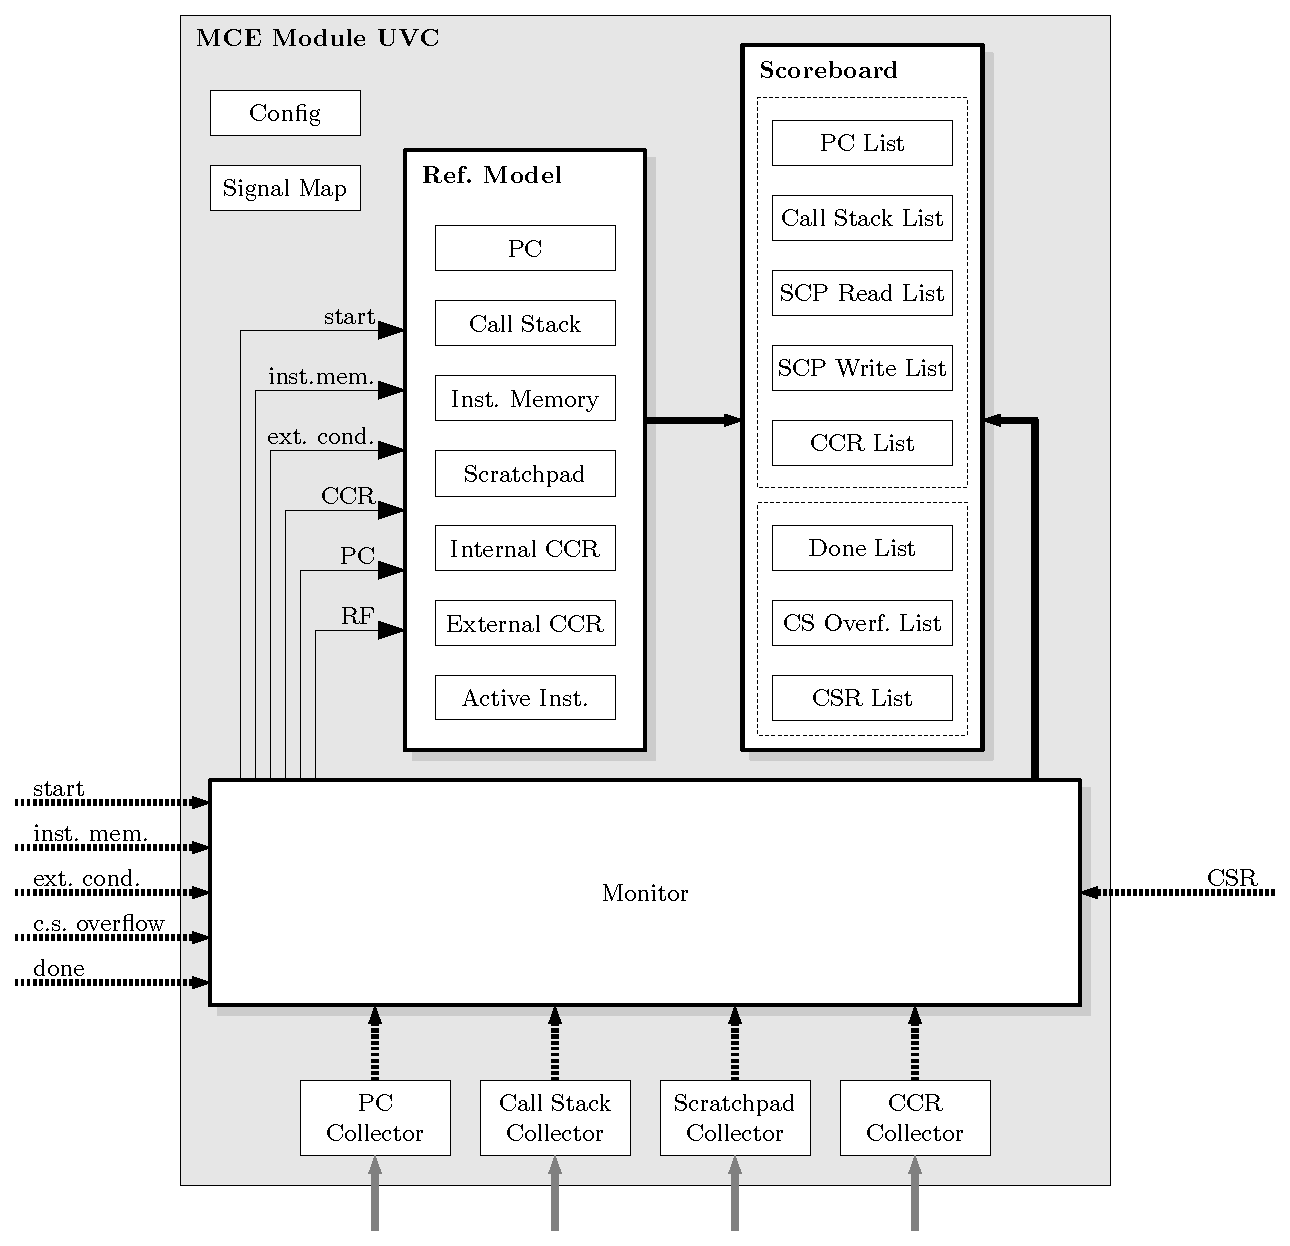
\includegraphics[scale=1.0]{images/mce_module_uvc}
 \caption{MCE Module UVC}
\label{fig:module_uvc}
\end{figure}

\subsubsection{Collectors}

\paragraph{Program Counter Collector}

\paragraph{Call Stack Collector}

\paragraph{Scratchpad Collector}

\paragraph{Condition Code Register Collector}

\subsubsection{Monitor}

\subsubsection{Scoreboard}

\subsubsection{Reference Model}

\paragraph{List of Active Instructions}

\paragraph{Instruction Execution Flow}

\paragraph{Stall Barrier}

\paragraph{Register File Read Transactions}

\paragraph{CCR Write Transactions}

\subsection{Test Library}